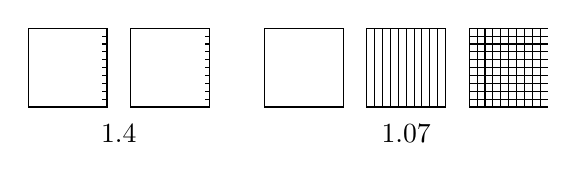
\begin{tikzpicture}[x=1cm,y=1cm]\foreach \x in {0,1.3}{\draw (\x,0) rectangle ++(1,1);\foreach \i in {1,...,9}{\draw (\x+1,.1*\i)--(\x+.94,.1*\i);}}\node[below] at (1.15,-.1){1.4};\draw (3,0) rectangle (4,1);\draw (4.3,0) rectangle (5.3,1);\foreach \i in {1,...,9}{\draw (4.3+.1*\i,0)--(4.3+.1*\i,1);}\draw[step=.1] (5.6,0) grid (6.6,1);\node[below] at (4.8,-.1){1.07};\end{tikzpicture}
